\documentclass[10pt, aspectratio=169]{beamer}
\usepackage{lmodern}
\usetheme{SimplePlus}
\usefonttheme{professionalfonts}
\usepackage{newtxtext}
\usepackage{newtxmath}
\usepackage{lmodern}
\usepackage{hyperref}
\usepackage{graphicx}
\usepackage{tcolorbox}
\usepackage{ragged2e}
\usepackage{tikz-cd}
\usepackage{tikz}
\usepackage{xcolor}
\usepackage{tcolorbox}
\usepackage[backend=biber]{biblatex}
\newcommand{\tb}{\textbf}
\newcommand{\ti}{\textit}
\bibliography{reference}


%--------------------------------------------------%

\title{Curvatura en variedades diferenciables y curvatura seccional en planos tangentes}

\author{Joan Sebastian Ramirez Sanchez}

\institute{ Departamento de Matemáticas \\
   Universidad del Valle}

%--------------------------------------------------%

\begin{document}

\begin{frame}
    \titlepage%
\end{frame}

%------------------------------------------------

%================================================
\section{Contexto biológico}
%================================================

\begin{frame}{Contexto biológico}
\begin{itemize}
    \item El mosquito \ti{Aedes aegypti} es el principal transmisor de dengue, Zika y chikungunya.
    \item \ti{Wolbachia} es la bacteria intracelular presente en muchos insectos. En los mosquitos reduce su capacidad de transmitir virus.
    \item La cepa \ti{wMelPop}
    \begin{itemize}
        \item[--] Es la que mejor actúa ante la reproducción del virus dentro del mosquito
        \item[--]Pero genera un \tb{alto costo biológico}: reduce la fecundidad de las hembras, la viabilidad de los huevos y la longevidad de los mosquitos infectados.
    \end{itemize}
    \item  Incompatibilidad citoplasma (\tb{CI}).
    Es un fenómeno reproductivo inducido por \ti{Wolbachia}
    \begin{itemize}
        \item[--] Cuando un macho infectado con \ti{Wolbachia} se aparea con una hembra no infectada, los huevos no eclosionan.
        \item[--] Cuando una hembra infectada se aparea con un macho no infectado, los huevos eclosionan normalmente y las crías heredan la infección.
    \end{itemize}
\end{itemize}

\end{frame}

\begin{frame}{Modelo de competencia entre hembras (sin control)}
\begin{itemize}
    \item \textbf{Variables de estado:}
    \begin{itemize}
        \item $F(t)$: número de hembras silvestres (no infectadas)
        \item $W(t)$: número de hembras portadoras de \textit{Wolbachia}
    \end{itemize}
    \item \textbf{Ecuaciones del modelo:}
    \begin{align*}
        \frac{dF}{dt} &= \left[\Psi_f - \frac{r_f}{K_f}(F+W)\right] F 
                         \left(\frac{F}{K_0} - 1\right) - \delta_f F,\\
        \frac{dW}{dt} &= \left[\Psi_w - \frac{r_w}{K_w}(F+W)\right] W 
                         - \delta_w W.
    \end{align*}
\end{itemize}

\end{frame}
\begin{frame}{Parámetros del modelo (I) – Natalidad y mortalidad}
\begin{itemize}
    \item $\Psi_f$, $\Psi_w$: tasas de \tb{nacimiento} de hembras adultas 
          (en ausencia de competencia) para las poblaciones silvestre e 
          infectada, respectivamente.
    \item $\delta_f$, $\delta_w$: tasas de \tb{mortalidad} natural de 
          hembras adultas.
    \item $r_f = \Psi_f - \delta_f$, \quad $r_w = \Psi_w - \delta_w$: 
          tasas intrínsecas de crecimiento (sin competencia).
    \item \textbf{Condición biológica:}  
          $\Psi_f > \Psi_w$ \quad y \quad $\delta_f < \delta_w$  
          $\Rightarrow$ las hembras silvestres son más fértiles y viven más 
          que las portadoras de \ti{wMelPop}.
    \item \textbf{Características principales:}
        \begin{itemize}
            \item El término $\left(\frac{F}{K_0}-1\right)$ introduce un 
              \textbf{efecto Allee} (depensación): cuando $F$ es baja, 
              las hembras silvestres tienen menos probabilidad de 
              encontrar parejas no infectadas y su reclutamiento se 
              vuelve negativo.
            \item El sistema posee un \textbf{umbral crítico} $K_{\flat}$ 
              (tamaño mínimo viable de $F$):
              \begin{itemize}
                  \item Si $F < K_{\flat}$, la población silvestre 
                        se extingue y la infección se fija.
                  \item Si $F > K_{\flat}$, las silvestres persisten 
                        y \textit{Wolbachia} desaparece.
        \end{itemize}
    \end{itemize}
    \end{itemize}
\end{frame}
%%%%%%%%%%%%%%%%%%%%%%%%%%%%%%%%%%%%%%%%%%%%%%%%%%%%%%%%%%%%%%%%%%%%%%%%%%%%%%%%%%%%%%%


%%%%%%%%%%%%%%%%%%%%%%%%%%%%%%%%%%%%%%%%%%%%%%%%%%%%%%%%%%%%%%%%%%%%%%%%%%%%%%%%%%%%%%%
\begin{frame}{Modelo de competencia entre hembras (con control)}
    El control $u(t)$ será el número de mosquitos con \ti{Wolbachia} liberados en un dia $t$ en 
    en el campo, así el sistema nos queda
    \begin{align*}
                \frac{dF}{dt} &= \left[\Psi_f - \frac{r_f}{K_f}(F+W)\right] F 
                         \left(\frac{F}{K_0} - 1\right) - \delta_f F,\\
        \frac{dW}{dt} &= \left[\Psi_w - \frac{r_w}{K_w}(F+W)\right] W 
                         - \delta_w W + u(t).
    \end{align*}
    con $u(t) \in [0, u_{\max}]$, con $u_{\max}$ la capacidad máxima 
              diaria de producción en laboratorio.
\end{frame}
\begin{frame}{Condiciones de frontera}
    tenemos que las condiciones de fronetera serán
    \begin{itemize}
        \item Inicio: $F(0) = K_f$ (densidad moderada de silvestres, 
              $K_f < K_{\flat}$), \; $W(0) = 0$.
        \item Meta: $F(T) = F_T < K$ (por debajo del umbral de extinción 
              $K_{\flat}$).
    \end{itemize}
\end{frame}
\begin{frame}{Objetivo de control: el funcional $\mathcal{J}(u,T)$}
\begin{itemize}
    \item \textbf{Propósito:} minimizar simultáneamente el \tb{tiempo total} 
          de intervención y el \tb{costo} de cría artificial de hembras 
          infectadas.
    \item \textbf{Funcional a minimizar:}
          \[
          \mathcal{J}(u,T) = \int_{0}^{T} \left(1 + \frac{C}{2}\, u^2(t)\right) dt
          \]
    \item \textbf{Componentes del integrando:}
          \begin{itemize}
              \item $1$: penaliza la duración del programa (cada día cuenta).
              \item $\displaystyle \frac{C}{2}\,u^2(t)$: penaliza el esfuerzo 
                    de liberación (costo cuadrático creciente).
          \end{itemize}
    \item \textbf{Tiempo terminal $T$ libre:} se determina de forma óptima 
          junto con $u^*(t)$.
    \item \textbf{Restricción terminal:} $F(T) = K_0 < K_{\flat}$.
\end{itemize}
\end{frame}
\begin{frame}{El parámetro $C$: balance entre tiempo y costo}
\begin{itemize}
    \item $C > 0$ refleja la \tb{importancia relativa} del costo de 
          producción frente a la urgencia temporal.
    \item \textbf{Dos escenarios de prioridad:}
          \begin{itemize}
              \item \textbf{Opción A:} $C = 0.01$ \\[2pt]
                    \textit{El tiempo es mucho más importante que el costo.}
              \item \textbf{Opción B:} $C = 1$ \\[2pt]
                    \textit{Ambos criterios (tiempo y costo) son igualmente importantes.}
          \end{itemize}
    \item \textbf{Efecto esperado:}
          \begin{itemize}
              \item Con $C$ pequeño (Opción A), el óptimo tiende a reducir 
                    $T^*$ aunque se libere más cada día.
              \item Con $C$ grande (Opción B), el óptimo tiende a ahorrar 
                    cría aunque la intervención dure más.
          \end{itemize}
\end{itemize}
\end{frame}
\begin{frame}{Principio del máximo de Pontryagin (I): Hamiltoniano}
\begin{itemize}
    \item Para aplicar el principio, se introduce el \tb{Hamiltoniano}:
    \begin{align*}
        H &= -1 - \frac{C}{2}u^2 \\
          &\quad + \lambda_1 \left[ \left(\Psi_f - \frac{r_f}{K_f}(F+W)\right) 
             F\left(\frac{F}{K_0}-1\right) - \delta_f F \right] \\
          &\quad + \lambda_2 \left[ \left(\Psi_w - \frac{r_w}{K_w}(F+W)\right) 
             W - \delta_w W + u \right].
    \end{align*}
    \item $\lambda_1(t)$, $\lambda_2(t)$: variables adjuntas (precios sombra 
          de $F$ y $W$).
    \item El Hamiltoniano reúne el costo instantáneo $(-1 - \frac{C}{2}u^2)$ 
          y la dinámica del sistema ponderada por los precios sombra.
\end{itemize}
\end{frame}

\begin{frame}{Principio del máximo de Pontryagin (II): Condición de maximalidad}
\begin{itemize}
    \item El control óptimo $u^*(t)$ debe maximizar $H$ en cada instante.
    \item Derivamos $H$ respecto a $u$:
          \[
          \frac{\partial H}{\partial u} = -C u + \lambda_2 = 0.
          \]
    \item Como la segunda derivada es negativa ($\partial^2 H / \partial u^2 = -C < 0$), 
          el punto crítico es un máximo.
    \item La condición anterior expresa la igualdad entre 
          \tb{costo marginal} ($C u$) y \tb{beneficio marginal} ($\lambda_2$).
\end{itemize}
\end{frame}

\begin{frame}{Principio del máximo de Pontryagin (III): Caracterización del control}
\begin{itemize}
    \item Teniendo en cuenta la cota $u(t) \in [0, u_{\max}]$, se obtiene:
          \[
          u^*(t) = \max\left\{0,\;\min\left\{\frac{\lambda_2(t)}{C},\; u_{\max}\right\}\right\}.
          \]
    \item \textbf{Interpretación directa:}
          \begin{itemize}
              \item Si $\lambda_2/C \le 0 \;\Rightarrow\; u^*=0$ (no conviene liberar).
              \item Si $0 < \lambda_2/C < u_{\max} \;\Rightarrow\; u^*=\lambda_2/C$ 
                    (liberación intermedia).
              \item Si $\lambda_2/C \ge u_{\max} \;\Rightarrow\; u^*=u_{\max}$ 
                    (liberación al máximo posible).
          \end{itemize}
    \item Esta expresión define el control óptimo en función del precio sombra 
          $\lambda_2$ y del costo relativo $C$.
\end{itemize}
\end{frame}
\begin{frame}{Interpretación económica del control óptimo}
\begin{itemize}
    \item $\lambda_2(t)$: \tb{beneficio marginal} de liberar una hembra infectada 
          adicional (en términos de acercar el sistema a la extinción de $F$).
    \item $C u(t)$: \tb{costo marginal} de liberar $u(t)$ hembras 
          (producción en laboratorio).
    \item \textbf{Regla de decisión:}
          \begin{itemize}
              \item Si $\lambda_2 > C u$ (beneficio $>$ costo) 
                    $\Rightarrow$ aumentar liberaciones, hasta $u_{\max}$ si es preciso.
              \item Si $\lambda_2 < C u$ (costo $>$ beneficio) 
                    $\Rightarrow$ reducir liberaciones, incluso a cero.
              \item En el óptimo: $\lambda_2 = C u^*$ 
                    (costo marginal = beneficio marginal).
          \end{itemize}
    \item \textbf{Forma típica del control:}
          \begin{itemize}
              \item Crece al inicio (beneficio alto).
              \item Se mantiene en $u_{\max}$ mientras la ventaja persiste.
              \item Decrece al final cuando el umbral ya casi se alcanza.
          \end{itemize}
\end{itemize}
\end{frame}
\begin{frame}{Forma de los controles óptimos y su efecto en la dinámica}
\begin{itemize}
    \item \textbf{Estrategias óptimas} (ver Fig. 8 y Fig. 10 del artículo):
    \begin{itemize}
        \item \textit{Opción A} ($C=0.01$): el control crece rápidamente hasta $u_{\max}$, 
              se mantiene allí y luego desciende de forma abrupta.
        \item \textit{Opción B} ($C=1$): el control aumenta lentamente, permanece en $u_{\max}$ 
              un período más corto y decrece suavemente.
    \end{itemize}
\end{itemize}
\begin{figure}
      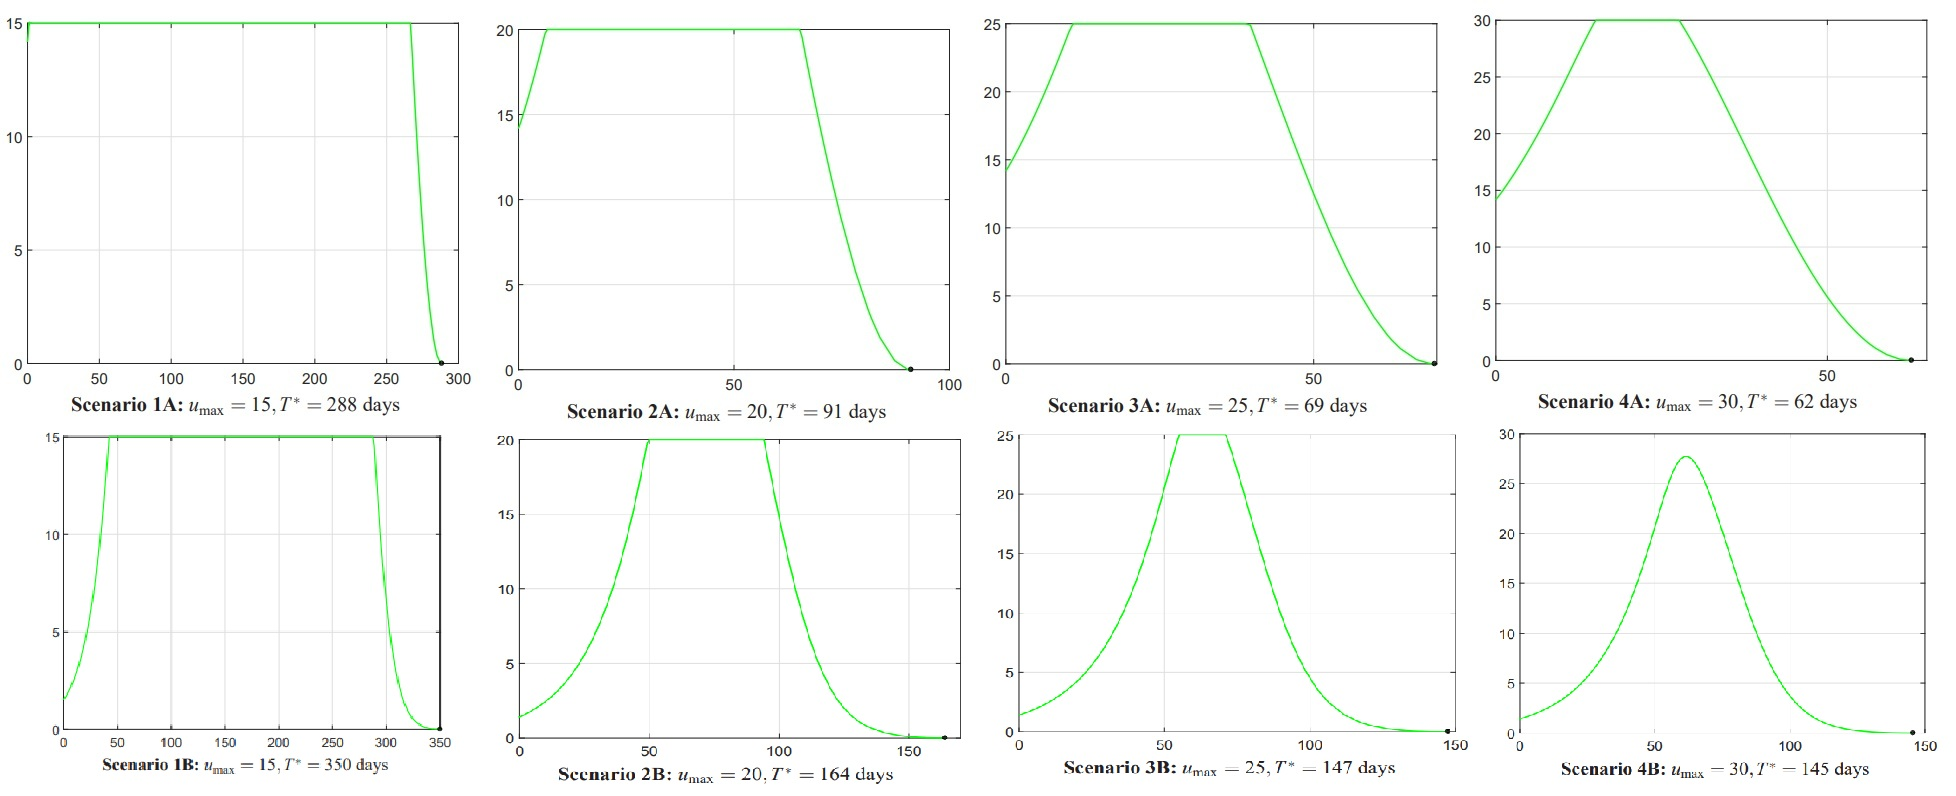
\includegraphics[width=12cm]{Sin título.jpg}
\end{figure}
\end{frame}
\begin{frame}{Forma de los controles óptimos y su efecto en la dinámica}
        \textbf{Trayectorias de las poblaciones} (ver Fig. 9 y Fig. 11):
          \begin{itemize}
        \item En todos los casos, $F^*(t)$ desciende hasta $F_T = K_0 < K_{\flat}$ al tiempo $T^*$.
        \item Con la Opción A, $F^*$ es convexa: cada liberación es efectiva.
        \item Con la Opción B, $F^*$ muestra un patrón cóncavo‑convexo: 
              parte del esfuerzo se pierde en competencia.
    \end{itemize}
\begin{figure}[h]
      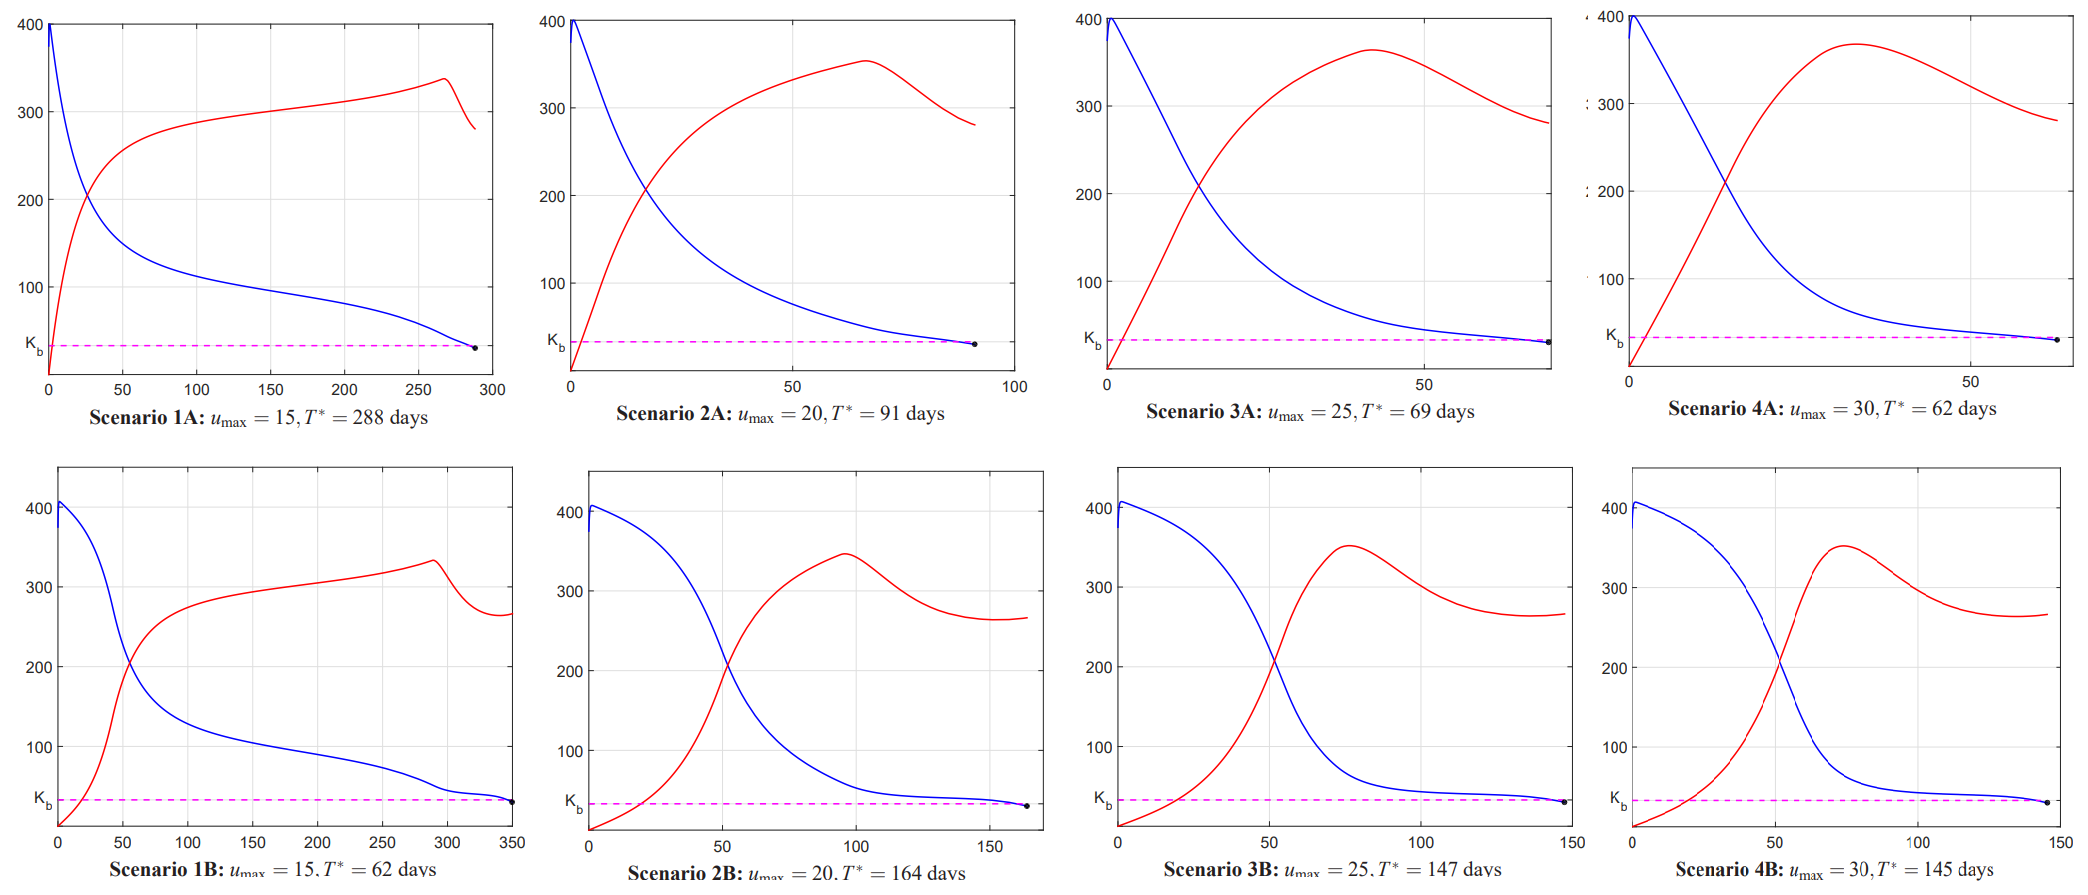
\includegraphics[width=12cm]{Sin título2.png}
\end{figure}
\end{frame}



\end{document}